
\documentclass[12pt]{article}
\usepackage[margin=1in]{geometry}
\usepackage{graphicx}
\usepackage{amsmath}
\usepackage{hyperref}

\title{ELCT 562 Q3}
\author{Jacob Vaught}
\date{\today}

\begin{document}

\maketitle

\subsection*{Solution}
In a wireless system with a 5 MHz bandwidth transmitted signal and a 2.1 GHz carrier frequency, the minimum required Digital-to-Analog Converter (DAC) sample rates for the in-phase and quadrature branches at the transmitter are determined to avoid aliasing. According to the Nyquist-Shannon sampling theorem, the minimum sampling frequency should be at least twice the maximum frequency of the signal. In this case, the minimum sampling rate for both the in-phase and quadrature components should be at least \textbf{5 Msps}.

Furthermore, if the DAC rate is set to 20 Msps, the guard band between aliases can be calculated. The guard band, which is the frequency range between the edge of the original signal’s spectrum and the start of the first alias, is found to be \textbf{17.5 MHz}. 

\subsection*{Frequency Spectrum Visualization}

% Include the generated plot here
\begin{figure}[h]
\centering
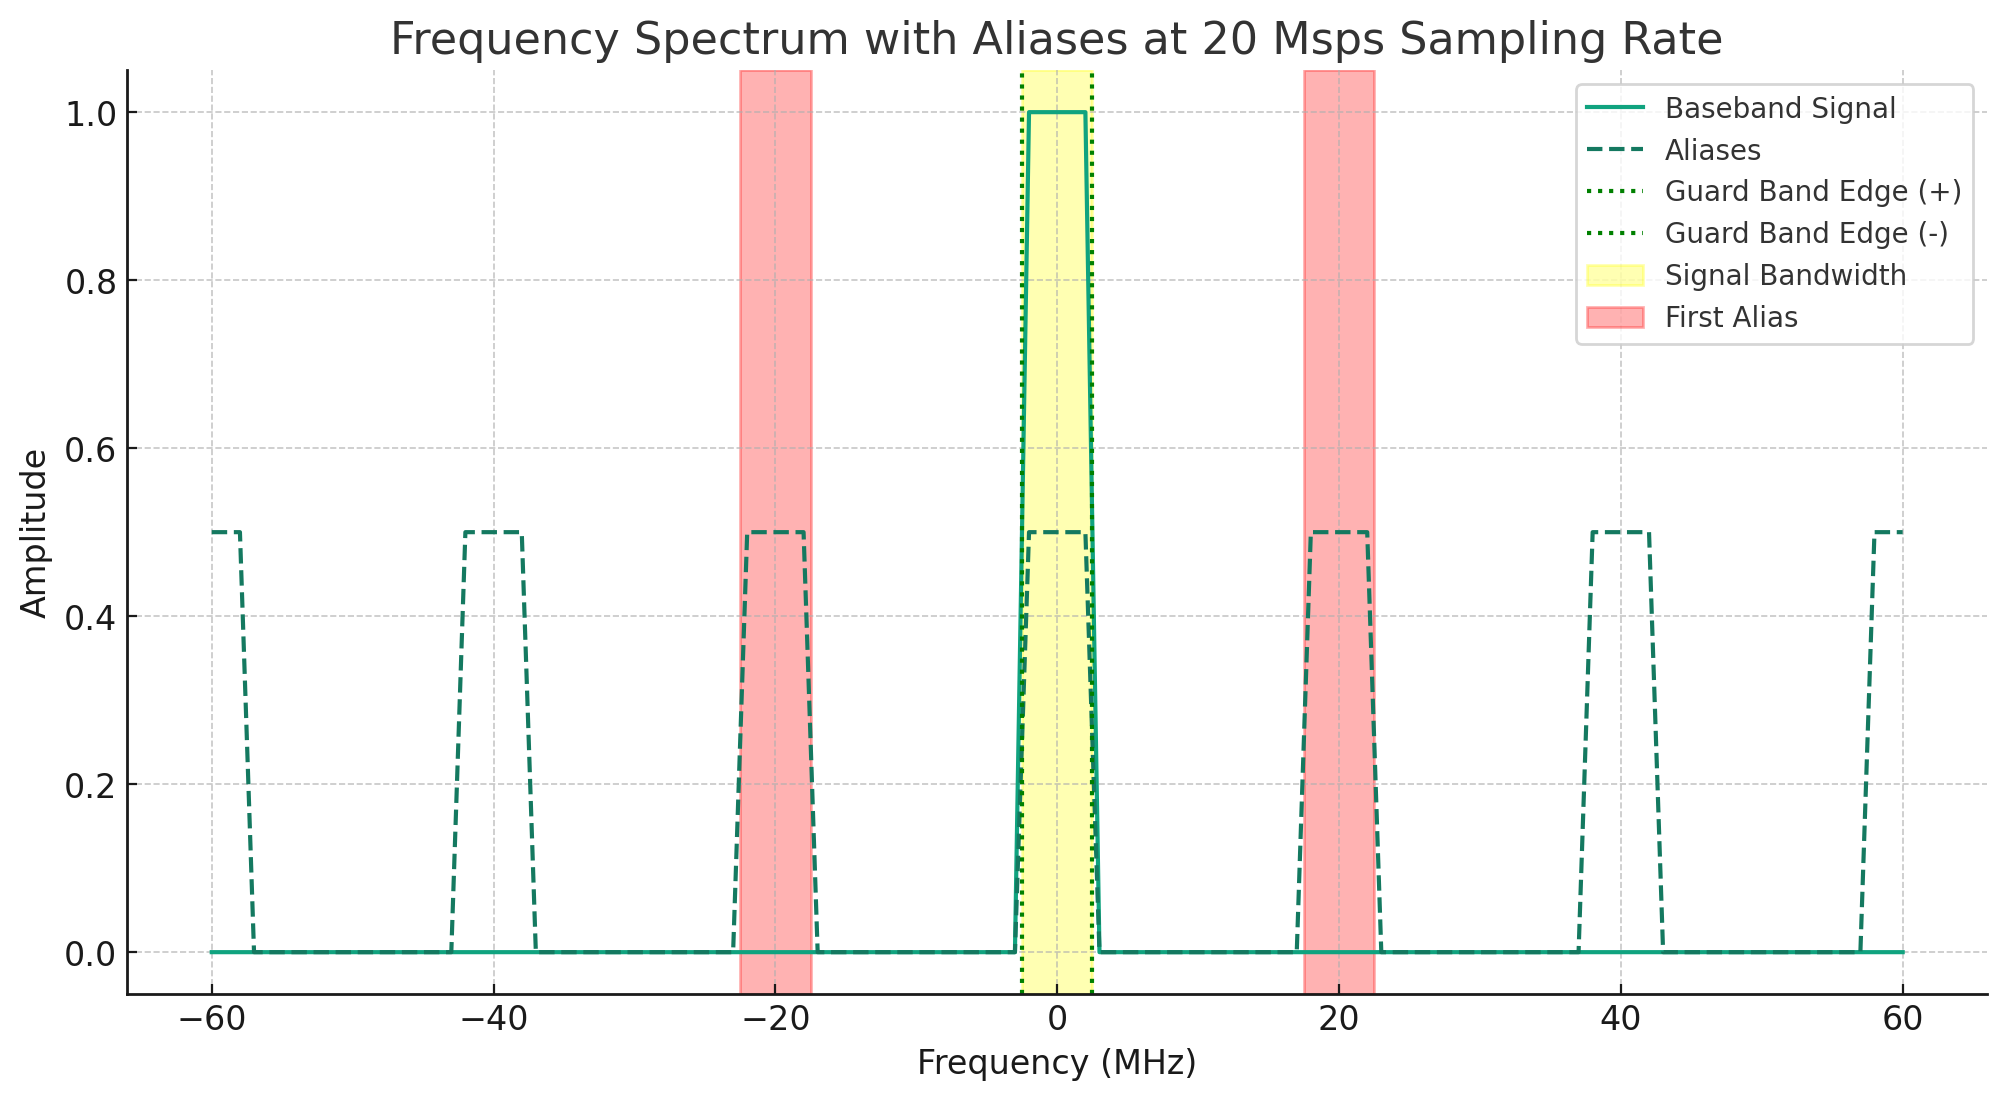
\includegraphics[width=0.8\textwidth]{frequency-spectrum.png}
\caption{Frequency spectrum with aliases at a 20 Msps sampling rate.}
\end{figure}

Note that the plot would be centered about 2.1 GHz, not 0.

\end{document}
